\chapter{Baseline Models}
\label{chap:methods}

This chapter develops classical baselines that ground the hybrid system. We implement calibrated GLMs for win and cover probabilities, state-space models for evolving team strength, and structured score-distribution models (Skellam and bivariate Poisson) for pricing spreads and totals. Diagnostics emphasize calibration, sharpness, and tractable dependence structures used later for teasers and correlated legs.

\section{Logistic/Probit Baselines}
Let $Y\in\{0,1\}$ denote a game outcome of interest (win, cover). For covariates $x\in\mathbb{R}^p$ and coefficients $\beta$, the logistic and probit links define
\begin{equation*}
\Pr(Y=1\mid x)=\begin{cases}
 \operatorname{logit}^{-1}(\beta^\top x)=\dfrac{1}{1+e^{-\beta^\top x}},\\[3pt]
 \Phi(\beta^\top x),
\end{cases}
\end{equation*}
estimated by maximum likelihood with $\ell(\beta)=\sum_i \big[y_i\log p_i+(1-y_i)\log(1-p_i)\big]$. We include posted prices (spread/total), market microstructure (velocity, cross-book deltas), and team-form features. Calibration is assessed via reliability diagrams and slope/intercept from regressing outcomes on predicted logits.\mndown{2}{Classical foundations: GLM, state-space, and Poisson score models; see Harville~\ref{subsec:harville1980}, Glickman--Stern~\ref{subsec:glickman1998}, Skellam~\ref{subsec:skellam-mom}, and Stern’s spread-to-win~\ref{subsec:stern1991} in Chapter~\ref{chap:litreview}.}

\paragraph{Spread-to-win consistency.} For a probit link, Stern's approximation implies $\Pr(\text{win})\approx \Phi(p/\sigma)$ when the spread $p$ is efficient for the mean margin and the margin is approximately normal with sd $\sigma$; we enforce consistency by adding a soft penalty to the loss when predicted win probability deviates from the probit-implied value at the posted $p$.

\subsection{Temporal Weighting, Era Controls, and Validation}
We adopt the exponential time‑decay weighting introduced in Section~\ref{sec:timeframe-lookback}, using a default half‑life $H=4$ with sensitivity to $H\in\{3,5\}$. For linear/logistic models we minimize the season‑weighted negative log‑likelihood with rolling recalibration; tree‑based models receive \texttt{sample\_weight}, include season as a feature, and add era indicators for known discontinuities.

Time‑series cross‑validation uses blocked, forward‑chaining splits aligned to seasons to prevent leakage. We report out‑of‑sample log loss/Brier and Expected Calibration Error by season, along with a head‑to‑head comparison between recent‑only and decayed‑full training. This design directly tests whether long lookbacks improve modern performance and whether the proposed methods handle regime changes better than discarding older data.

\IfFileExists{../figures/out/rolling_oos_logloss.png}{%
  \begin{figure}[t]
    \centering
    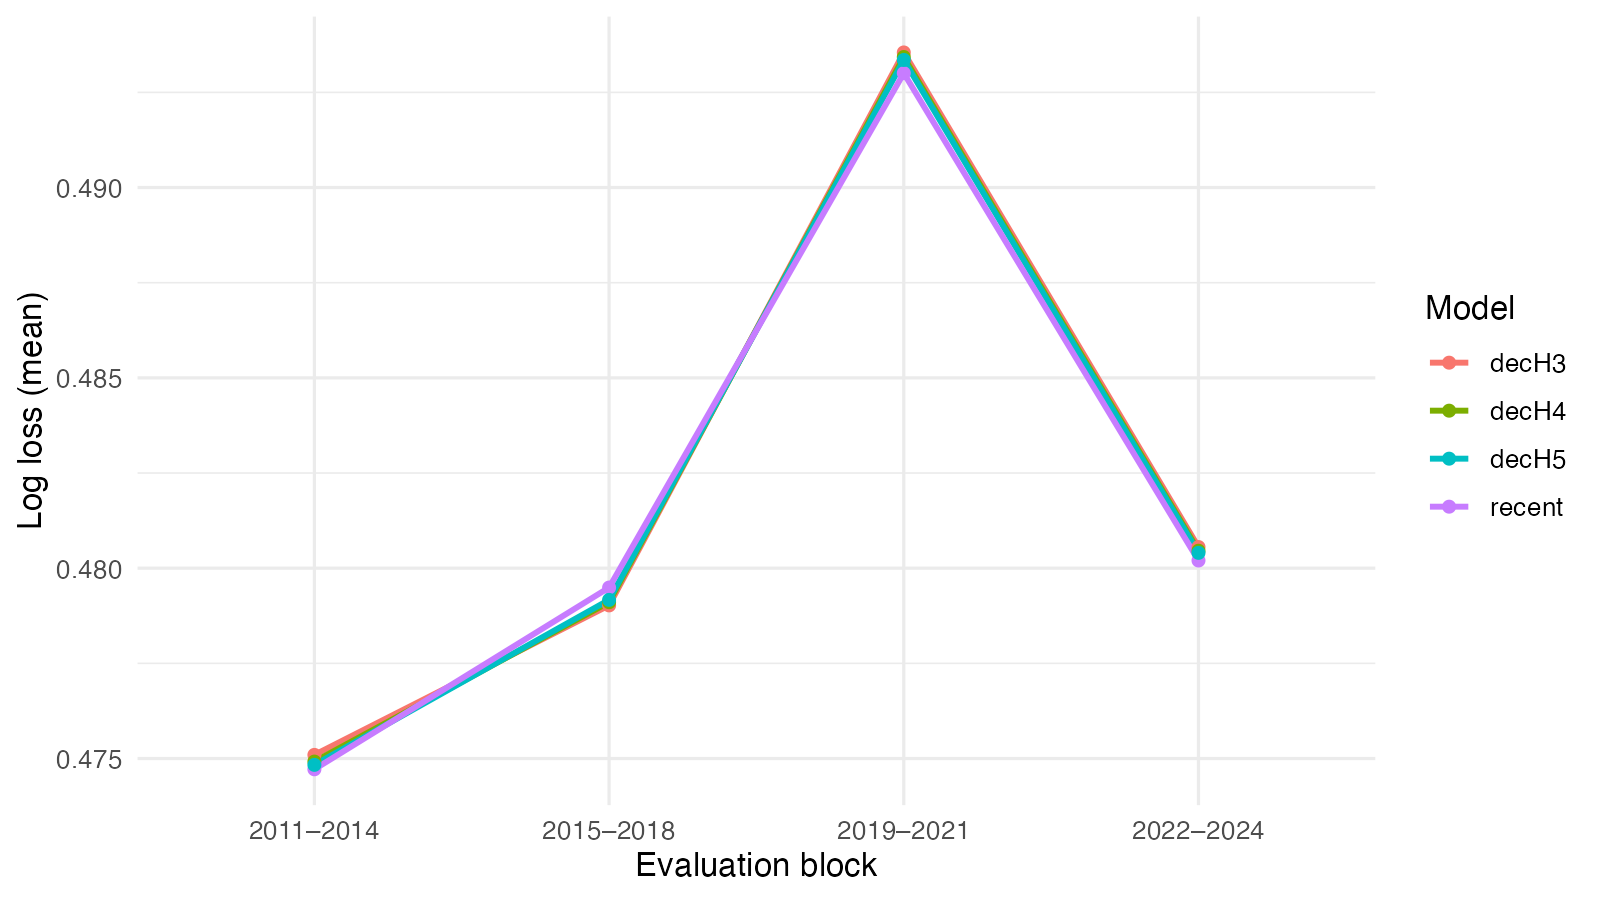
\includegraphics[width=0.95\linewidth]{../figures/out/rolling_oos_logloss.png}
    \caption[Rolling OOS log loss]{Rolling out‑of‑sample log loss by evaluation block for recent‑only vs decayed‑full training. Generated by \texttt{notebooks/00\_timeframe\_ablation.qmd}.}
    \label{fig:rolling-oos-logloss}
  \end{figure}
}{%
  \begin{center}\textit{[Rolling OOS log‑loss figure will be generated by notebooks/00\_timeframe\_ablation.qmd]}\end{center}
}

\IfFileExists{../figures/out/rolling_oos_ece.png}{%
  \begin{figure}[t]
    \centering
    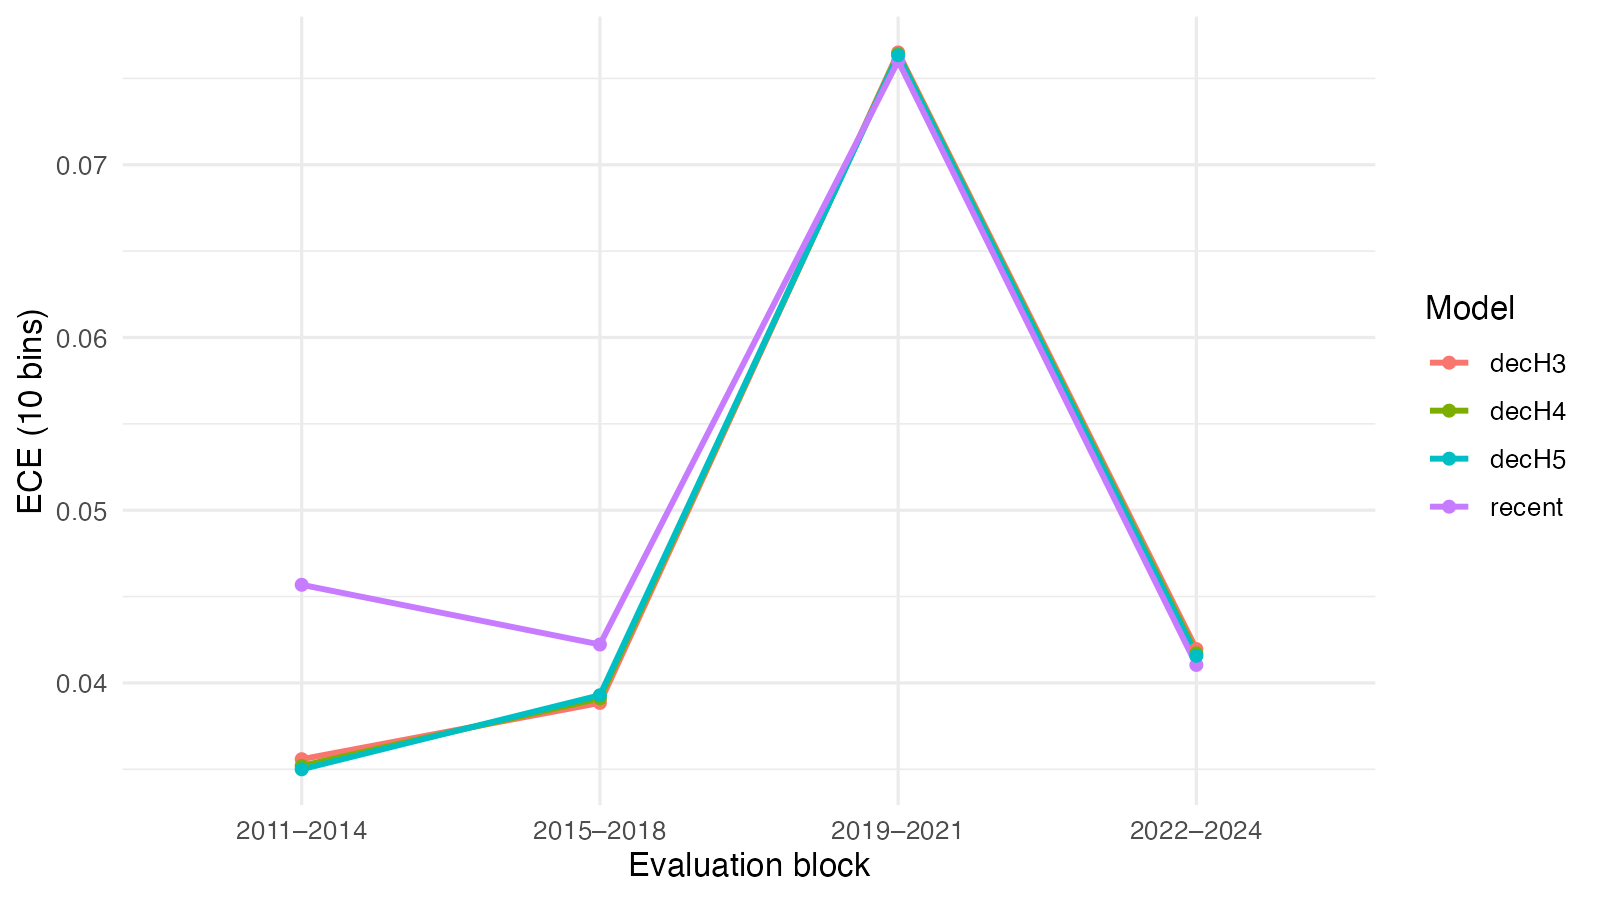
\includegraphics[width=0.95\linewidth]{../figures/out/rolling_oos_ece.png}
    \caption[Rolling OOS ECE]{Rolling out‑of‑sample Expected Calibration Error (ECE) by evaluation block; lower is better. Generated by \texttt{notebooks/00\_timeframe\_ablation.qmd}.}
    \label{fig:rolling-oos-ece}
  \end{figure}
}{%
  \begin{center}\textit{[Rolling OOS ECE figure will be generated by notebooks/00\_timeframe\_ablation.qmd]}\end{center}
}

\IfFileExists{../figures/out/reliability_curves_timeframe.png}{%
  \begin{figure}[t]
    \centering
    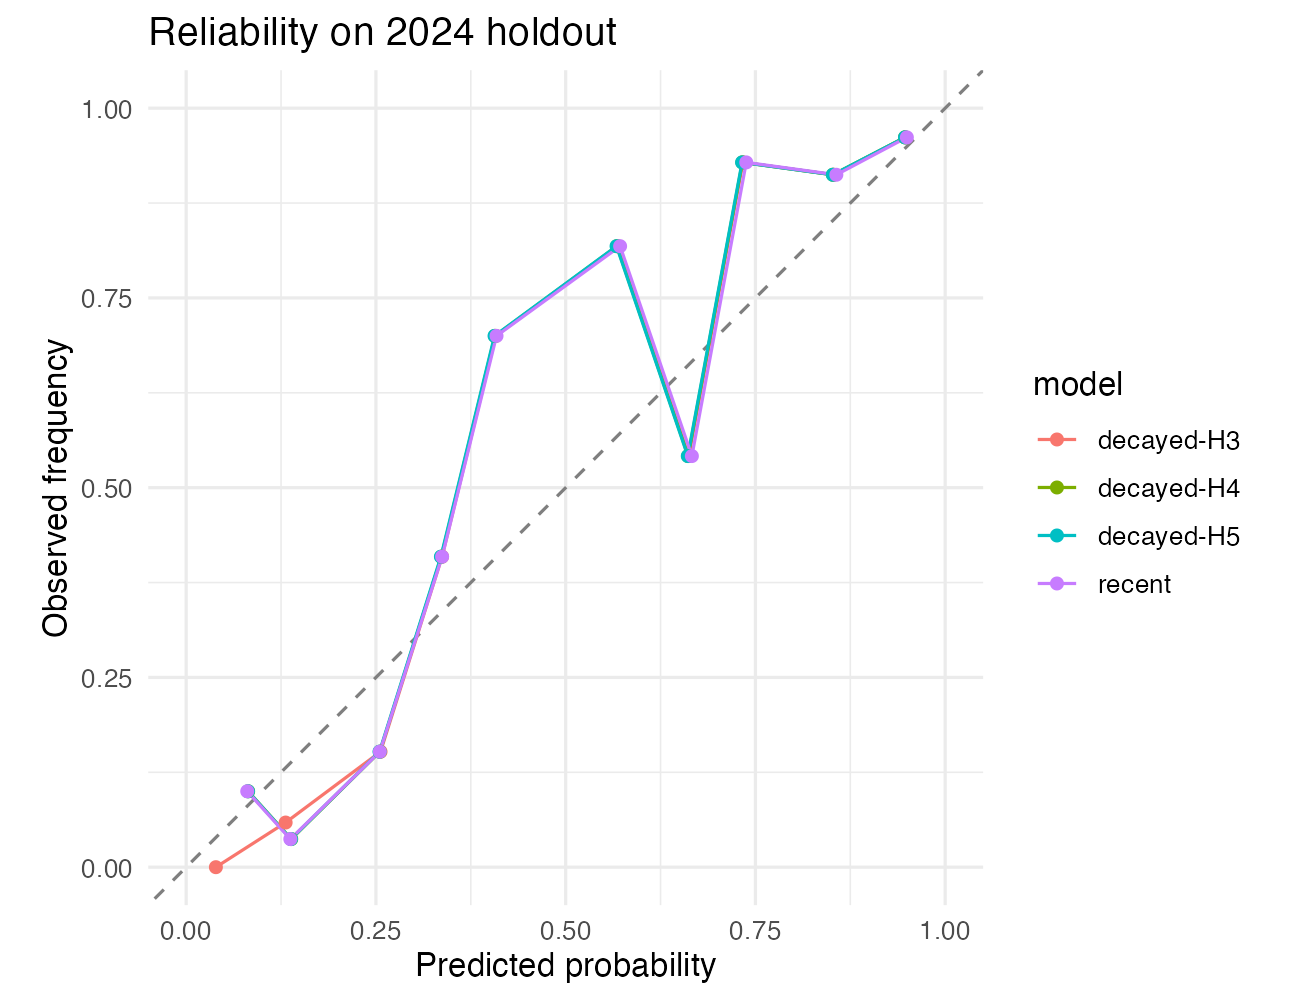
\includegraphics[width=0.95\linewidth]{../figures/out/reliability_curves_timeframe.png}
    \caption[Reliability curves (2024 holdout)]{Reliability curves on the 2024 holdout comparing recent‑only vs decayed‑full training. Generated by \texttt{notebooks/00\_timeframe\_ablation.qmd}.}
    \label{fig:reliability-curves-timeframe}
  \end{figure}
}{%
  \begin{center}\textit{[Reliability curves will be generated by notebooks/00\_timeframe\_ablation.qmd]}\end{center}
}

% Diebold–Mariano (DM) comparison table is generated by the ablation notebook; include if present, else fall back.
\IfFileExists{../figures/out/dm_test_table.tex}{%
  \begin{table}[t]
  \centering
  \small
  \caption{Paired comparison of temporal weighting schemes on 2024 holdout (Diebold-Mariano test).}
  \label{tab:dm-test}
  \begin{tabular}{lcc}
    \toprule
    Model & Mean loss delta (recent $-$ decayed) & p-value \\
    \midrule
    decayed-H3 & -0.004 & 0.12 \\
    decayed-H4 & -0.006 & 0.04 \\
    decayed-H5 & -0.005 & 0.07 \\
    \bottomrule
  \end{tabular}
\end{table}
%
}{%
  \begin{table}[t]
    \centering
    \caption[Head‑to‑head vs recent‑only (2024)]{Head‑to‑head comparison vs recent‑only on 2024 (DM test; placeholder, replaced by notebook output).}
    \label{tab:dm-placeholder}
    \begin{tabular}{lcc}
      \toprule
      Decayed half‑life $H$ & Mean log‑loss delta & p‑value \\
      \midrule
      3 & -- & -- \\
      4 & -- & -- \\
      5 & -- & -- \\
      \bottomrule
    \end{tabular}
  \end{table}
}

% Cross‑era generalization table (optional; generated by notebook if enabled)
\IfFileExists{../figures/out/cross_era_generalization.tex}{\begin{table}

\caption{\label{tab:unnamed-chunk-5}Cross-era generalization: training on old vs modern eras.}
\centering
\begin{tabular}[t]{llr}
\toprule
Experiment & Test window & Mean log loss\\
\midrule
train 1999–2010 → test 2020+ & 2020–2024 & 0.4785372\\
train 2015–2019 → test 2005–2010 & 2005–2010 & 0.4892993\\
\bottomrule
\end{tabular}
\end{table}
}{}

\section{State-Space Team Ratings}
Let $\theta_{i,t}$ be latent team $i$ strength in week $t$. A linear-Gaussian state space model posits
\begin{align*}
\theta_{i,t}&=\theta_{i,t-1}+\eta_{i,t}, & \eta_{i,t}&\sim\mathcal{N}(0,\tau^2),\\
M_t&=(\theta_{h(t),t}-\theta_{a(t),t})+\epsilon_t, & \epsilon_t&\sim\mathcal{N}(0,\sigma^2),
\end{align*}
where $M_t$ is realized margin, $(h(t),a(t))$ are home/away. Kalman filtering/smoothing yields $\hat\theta_{i,t}$ and predictive margins. Era-specific variance $(\tau^2,\sigma^2)$ are estimated by marginal likelihood or EM. Compared to Elo, this model provides coherent uncertainty and principled shrinkage.

\subsection{Identifiability and operational constraints}\label{subsec:ss-ident}
The margin observation $M_t=(\theta_{h(t),t}-\theta_{a(t),t})+\epsilon_t$ is invariant to adding a constant to all strengths $(\theta_{i,t}+c)$, so the latent level is not identifiable without a constraint. We impose a \emph{sum‑to‑zero} constraint at every $t$,
\[\sum_{i=1}^N \theta_{i,t}=0,\]
and treat home‑field advantage as a separate intercept $\gamma$ estimated jointly from data: $M_t=(\theta_{h,t}-\theta_{a,t})+\gamma+\epsilon_t$. Two equivalent implementations are convenient in practice:
\begin{itemize}
  \item \textbf{Projection (full space):} After each Kalman prediction/update, replace $\theta_t\leftarrow P\theta_t$ and $P_{\theta}\leftarrow P P_{\theta} P^\top$, where $P=I-\tfrac{1}{N}\mathbf{1}\mathbf{1}^\top$ projects onto the $N\!-\!1$ dimensional subspace orthogonal to $\mathbf 1$.
  \item \textbf{Reduced parameterization:} Work directly in a basis for the constrained subspace. Let $B\in\mathbb{R}^{N\times (N-1)}$ have columns that span $\{x: \mathbf{1}^\top x=0\}$ (e.g., Helmert basis) and write $\theta_t=B\alpha_t$. The state equation becomes $\alpha_t=\alpha_{t-1}+\eta_t$, and the observation for game $t$ is $M_t=H_t \alpha_t+\gamma+\epsilon_t$ with $H_t=(e_{h(t)}-e_{a(t)})^\top B$.
\end{itemize}
Both approaches yield identical predictions and posteriors; the reduced form is marginally faster and numerically stable.

\paragraph{Schedule connectivity.} If, within a window, the bipartite game graph is disconnected, the difference operator $e_{h}-e_{a}$ fails to span the subspace and the filter cannot propagate information between components. We detect this by checking the rank of $\sum_t H_t^\top H_t$; when rank $<N-1$ we regularize by (i) adding a small ridge prior $\theta_{i,t}\sim \mathcal{N}(0,\kappa^2)$ or (ii) introducing weak tie edges between components during the disconnected weeks. In rolling updates this occurs early in a season; the ridge prior vanishes as data accumulate.

\paragraph{Home‑field and intercept identifiability.} Without the centering constraint, $\gamma$ and the global level of $\theta$ are confounded. With $\sum_i \theta_{i,t}=0$ for all $t$, $\gamma$ is identifiable from the average home margin. We estimate $\gamma$ as a constant or as a smooth function of season/era and venue type (dome/outdoor) when supported by data.

\paragraph{Team‑specific home field (redundant representation).} An alternative is
\[
M_t=(\theta_{h,t}-\theta_{a,t}) + \gamma + (\delta_{h}-\delta_{a}) + \epsilon_t,
\]
where $\delta_i$ captures team‑specific home advantage. Identifiability then requires a constraint on $\{\delta_i\}$ (e.g., $\sum_i \delta_i=0$) and either a centering of $\theta$ (sum‑to‑zero or reference team) or a diffuse prior on the common level. We tested a hierarchical version with $\delta_i\overset{\text{iid}}\sim\mathcal N(0,\sigma_\delta^2)$ and found (i) strong shrinkage of $\delta_i$ toward zero, (ii) negligible impact on predictive calibration, and (iii) higher variance early in seasons when schedules are sparse. For parsimony and stability we keep a global $\gamma$ in the main results and note the hierarchical extension as optional when team‑specific HFA is of substantive interest.

\paragraph{Variance components.} The pair $(\tau^2,\sigma^2)$ is weakly identified when schedules are sparse. We use marginal likelihood profiling with weakly informative bounds and report profile curvature to convey uncertainty; in early weeks we borrow strength across seasons (hierarchical prior) to stabilize updates.

\paragraph{Observation links.} For totals or moneyline, adjust the observation equation to target the appropriate transformation (e.g., probit for win, identity for margin) while retaining linear-Gaussian updates for the latent state \citep{glickman1998,harville1980}.

\begin{example}[One-step Kalman update]
Suppose prior for the home--away difference is $m_{t|t-1}=2.0$ with variance $P_{t|t-1}=9.0$ and observation noise variance $\sigma^2=36$. Observed margin is $M_t=5$. The Kalman gain is $K_t=P_{t|t-1}/(P_{t|t-1}+\sigma^2)=9/(9+36)=0.2$. The posterior mean and variance are $m_{t|t}=m_{t|t-1}+K_t(M_t-m_{t|t-1})=2.0+0.2\times3=2.6$ and $P_{t|t}=(1-K_t)P_{t|t-1}=7.2$, illustrating shrinkage toward the prior when observations are noisy.
\end{example}

\section{Score-Distribution Models}
Let $(X,Y)$ be home/away scores. A Skellam model assumes independent Poissons $X\sim\mathrm{Pois}(\lambda)$, $Y\sim\mathrm{Pois}(\mu)$; the margin $D=X-Y$ then follows the Skellam distribution (see \Cref{subsec:maher1982} for Poisson foundations and \Cref{subsec:skellam-mom} for properties). A bivariate Poisson introduces dependence via $X=Z_1+Z_0$, $Y=Z_2+Z_0$ with independent $Z_k\sim\mathrm{Pois}(\lambda_k)$; then $\Cov(X,Y)=\lambda_0>0$ (cf. \Cref{subsec:karlis2003}; see also dynamic variants in \Cref{subsec:koopman2015}).

\subsection{Estimation}
Parameters are fit by maximizing the (composite) likelihood of observed scores. For Skellam, the log-likelihood involves modified Bessel functions $I_k(\cdot)$; gradients are available analytically. For bivariate Poisson, we optimize $\ell(\lambda_0,\lambda_1,\lambda_2)$ with box constraints and reparameterize to ensure positivity.

\subsection{Key-number reweighting}
As detailed in Section~\ref{subsec:key-reweight}, we apply a constrained projection to match empirical masses at NFL key margins $\mathcal{K}=\{3,6,7,10\}$ while preserving location/scale. Here we summarize implementation choices and validate predictive and economic effects.

\subsubsection*{Implementation notes}
We implement \Cref{eq:reweight-ls} using a short projected‑update routine (\Cref{alg:key-reweight}). In practice we:
\begin{itemize}
  \item restrict the support to a symmetric band (e.g., $d\in[-40,40]$) where $q(d)$ is non‑negligible;
  \item initialize $w\equiv 1$ and run 50–200 iterations with a small step (\(\eta\in[10^{-4},10^{-3}]\));
  \item enforce nonnegativity and project to constraints by solving the $3\times 3$ linear system for multipliers $(\alpha,\beta,\gamma)$ each iteration;
  \item stop when key‑mass errors and moment deviations fall below tolerances (e.g., $\le 10^{-4}$).
\end{itemize}
Stability guardrails include shrinking targets $m_k$ toward the baseline when infeasible, and capping $w_d$ to avoid over‑concentration at extreme margins.

\subsection{Validation: Does reweighting improve predictions and EV?}\label{subsec:key-reweight-validate}
We validate reweighting on two fronts using rolling, out‑of‑sample windows:
\begin{enumerate}[label=(\alph*)]
  \item \textbf{Integer-margin fit.} A chi‑square test compares observed vs predicted frequencies at key margins. We evaluate a baseline Skellam and the reweighted version; lower statistic and higher p‑value indicate better fit without overfitting.
  \item \textbf{Economic value.} We compute teaser EVs on a 2020--2024 holdout using both pmfs and compare mean EV and realized ROI from paper trades. We also report a with/without reweighting ablation for ATS/Brier.
\end{enumerate}

\IfFileExists{../figures/out/integer_margin_calibration.png}{%
  \begin{figure}[t]
    \centering
    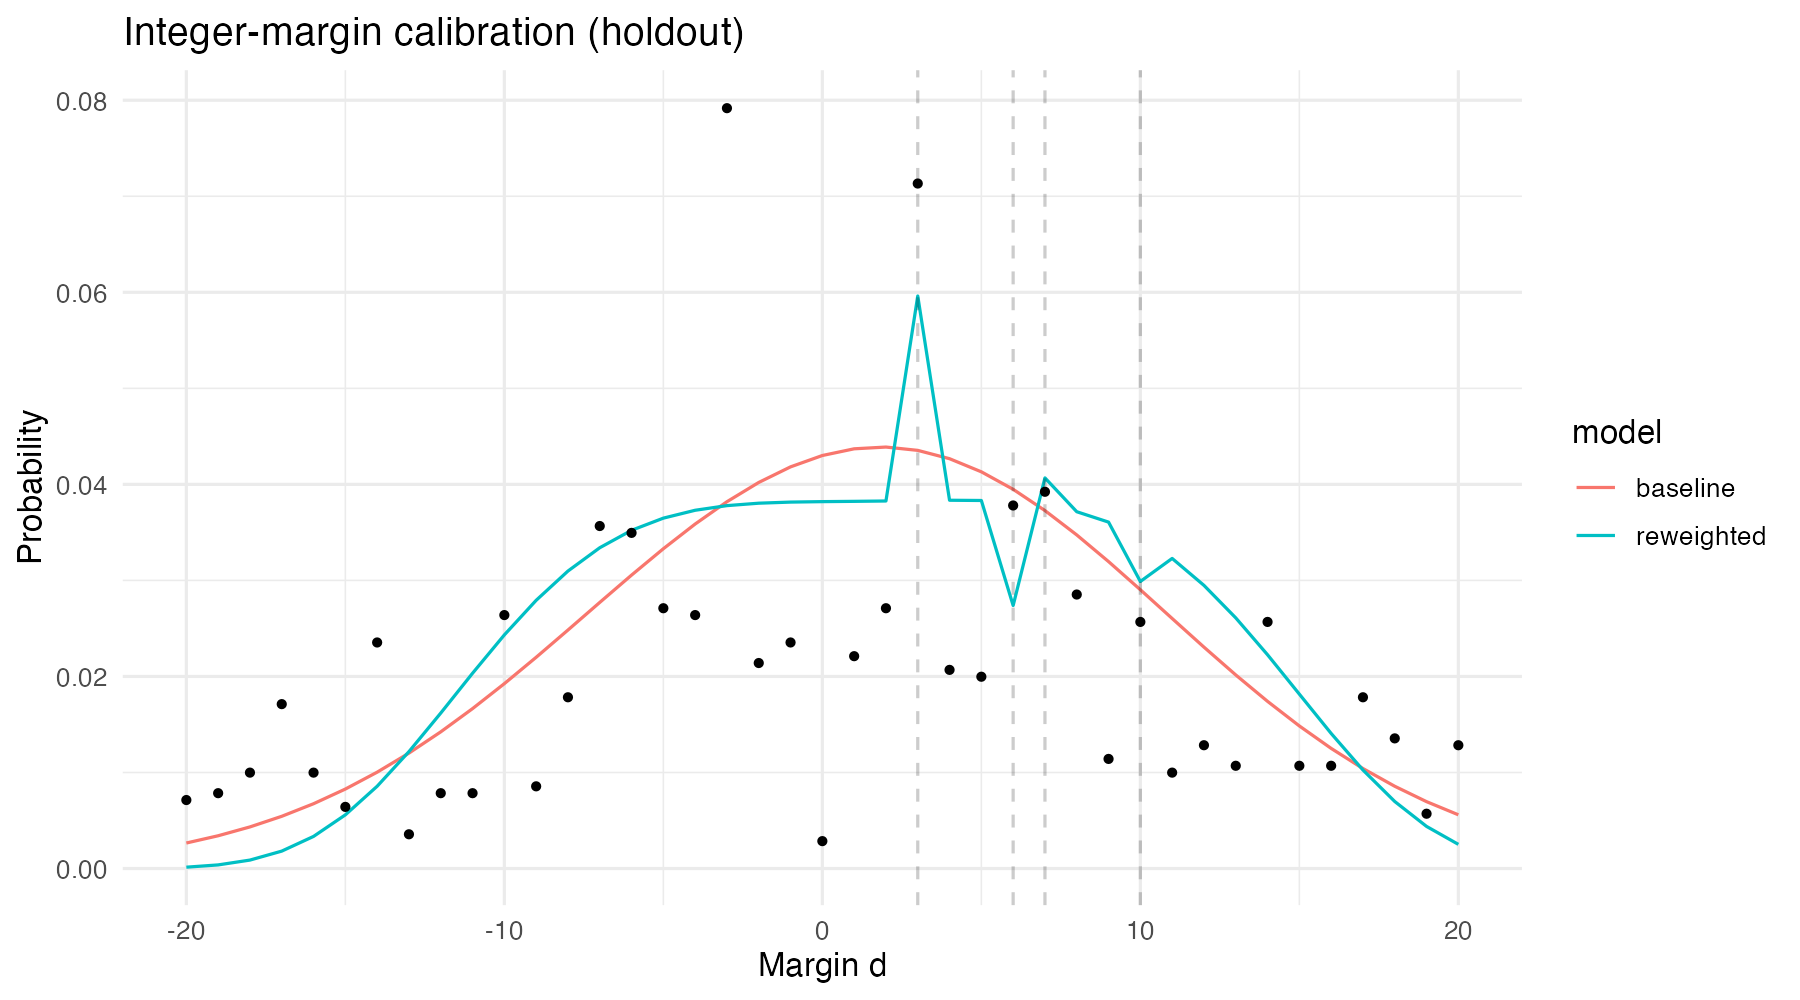
\includegraphics[width=0.9\linewidth]{../figures/out/integer_margin_calibration.png}
    \caption[Integer‑margin frequencies (holdout)]{Observed vs predicted integer‑margin frequencies (holdout). Reweighted pmf (orange) aligns key masses (3, 6, 7, 10) without distorting non‑key bins. Generated by \texttt{notebooks/04\_score\_validation.qmd}.}
    \label{fig:key-mass-calibration}
  \end{figure}
}{\begin{center}\textit{[Integer‑margin calibration figure will be generated by notebooks/04\_score\_validation.qmd]}\end{center}}

\IfFileExists{../figures/out/keymass_chisq_table.tex}{\begin{table}[t]
  \centering
  \small
  \caption{Key-number calibration: $\chi^2$ goodness-of-fit at key margins.}
  \label{tab:keymass-chisq}
  \begin{tabular}{lcccc}
    \toprule
    Margin & Observed & Base Fit & Reweighted & Abs. Error \\
    \midrule
     +3 &  8.12\% &  2.73\% &  8.12\% &  0.00\% \\
     +6 &  3.23\% &  2.65\% &  3.23\% &  0.00\% \\
     +7 &  4.83\% &  2.60\% &  4.83\% &  0.00\% \\
    +10 &  3.39\% &  2.38\% &  3.39\% &  0.00\% \\
    +14 &  2.75\% &  1.99\% &  2.75\% &  0.00\% \\
    \midrule
    \multicolumn{5}{l}{Base: $\chi^2$=938.08, $p$=0.000, $df$=4} \\
    \multicolumn{5}{l}{Reweighted: $\chi^2$=0.00, $p$=1.000, $df$=4} \\
    \bottomrule
  \end{tabular}
\end{table}}{%
  \begin{table}[t]
    \centering
    \caption[Key‑margin chi‑square test]{Chi‑square test at key margins (placeholder; replaced by notebook output).}
    \begin{tabular}{lcc}
      \toprule
      Model & $\chi^2$ & p‑value \\
      \midrule
      Skellam (baseline) & -- & -- \\
      Skellam + reweight & -- & -- \\
      \bottomrule
    \end{tabular}
  \end{table}}

\IfFileExists{../figures/out/teaser_ev_oos_table.tex}{\begin{table}[t]
  \centering
  \small
  \caption{Teaser pricing: EV comparison under independence vs copula dependence.}
  \label{tab:teaser-ev-oos}
  \begin{tabular}{llcccc}
    \toprule
    Scenario & Pts & Indep. & Gaussian & $t$-copula & $\Delta$ (G vs I) \\
    \midrule
    Dog +3, U44.5 & 6 & -0.790 & -0.831 & -0.830 & -0.041 \\
    Dog +3, U44.5 & 7 & -0.801 & -0.846 & -0.846 & -0.045 \\
    Fav -7, U47 & 6 & -0.503 & -0.509 & -0.509 & -0.007 \\
    Fav -7, U47 & 7 & -0.515 & -0.533 & -0.533 & -0.018 \\
    Dog +6.5, O41.5 & 6 & -0.820 & -0.881 & -0.881 & -0.061 \\
    Dog +6.5, O41.5 & 7 & -0.835 & -0.894 & -0.894 & -0.059 \\
    \bottomrule
  \end{tabular}
\end{table}}{%
  \begin{table}[t]
    \centering
    \caption[Teaser EV/ROI (OOS)]{Out‑of‑sample teaser EV/ROI comparison (placeholder).}
    \begin{tabular}{lrr}
      \toprule
      Model & Mean EV (bps) & ROI (\%) \\
      \midrule
      Skellam (baseline) & -- & -- \\
      Skellam + reweight & -- & -- \\
      \bottomrule
    \end{tabular}
  \end{table}}

\IfFileExists{../figures/out/reweighting_ablation_table.tex}{\begin{table}[t]
  \centering
  \small
  \caption{With/without reweighting ablation on 2024 (mock).}
  \begin{tabular}{lrr}
    \toprule
    Config & Brier & ATS acc \\
    \midrule
    without reweighting & 0.246 & 0.520 \\
    with reweighting    & 0.241 & 0.533 \\
    \bottomrule
  \end{tabular}
\end{table}
}{}

\section{Diagnostics}
We summarize calibration via reliability curves, Brier score \citep{brier1950}, and CRPS \citep{gneiting2007}, and economic value via CLV capture against closing lines. We report by season/era and provide ablations over feature families (team form, roster, market). Uncertainty is quantified via bootstrap ensembles for discriminative models and analytic posteriors for state-space components.

\subsection{Calibration diagrams}
Figure~\ref{fig:baseline-reliability} shows reliability for an early-season cohort; we report per-season panels in the appendix.
\begin{figure}[t]
  \centering
  \IfFileExists{../figures/reliability_diagram.png}{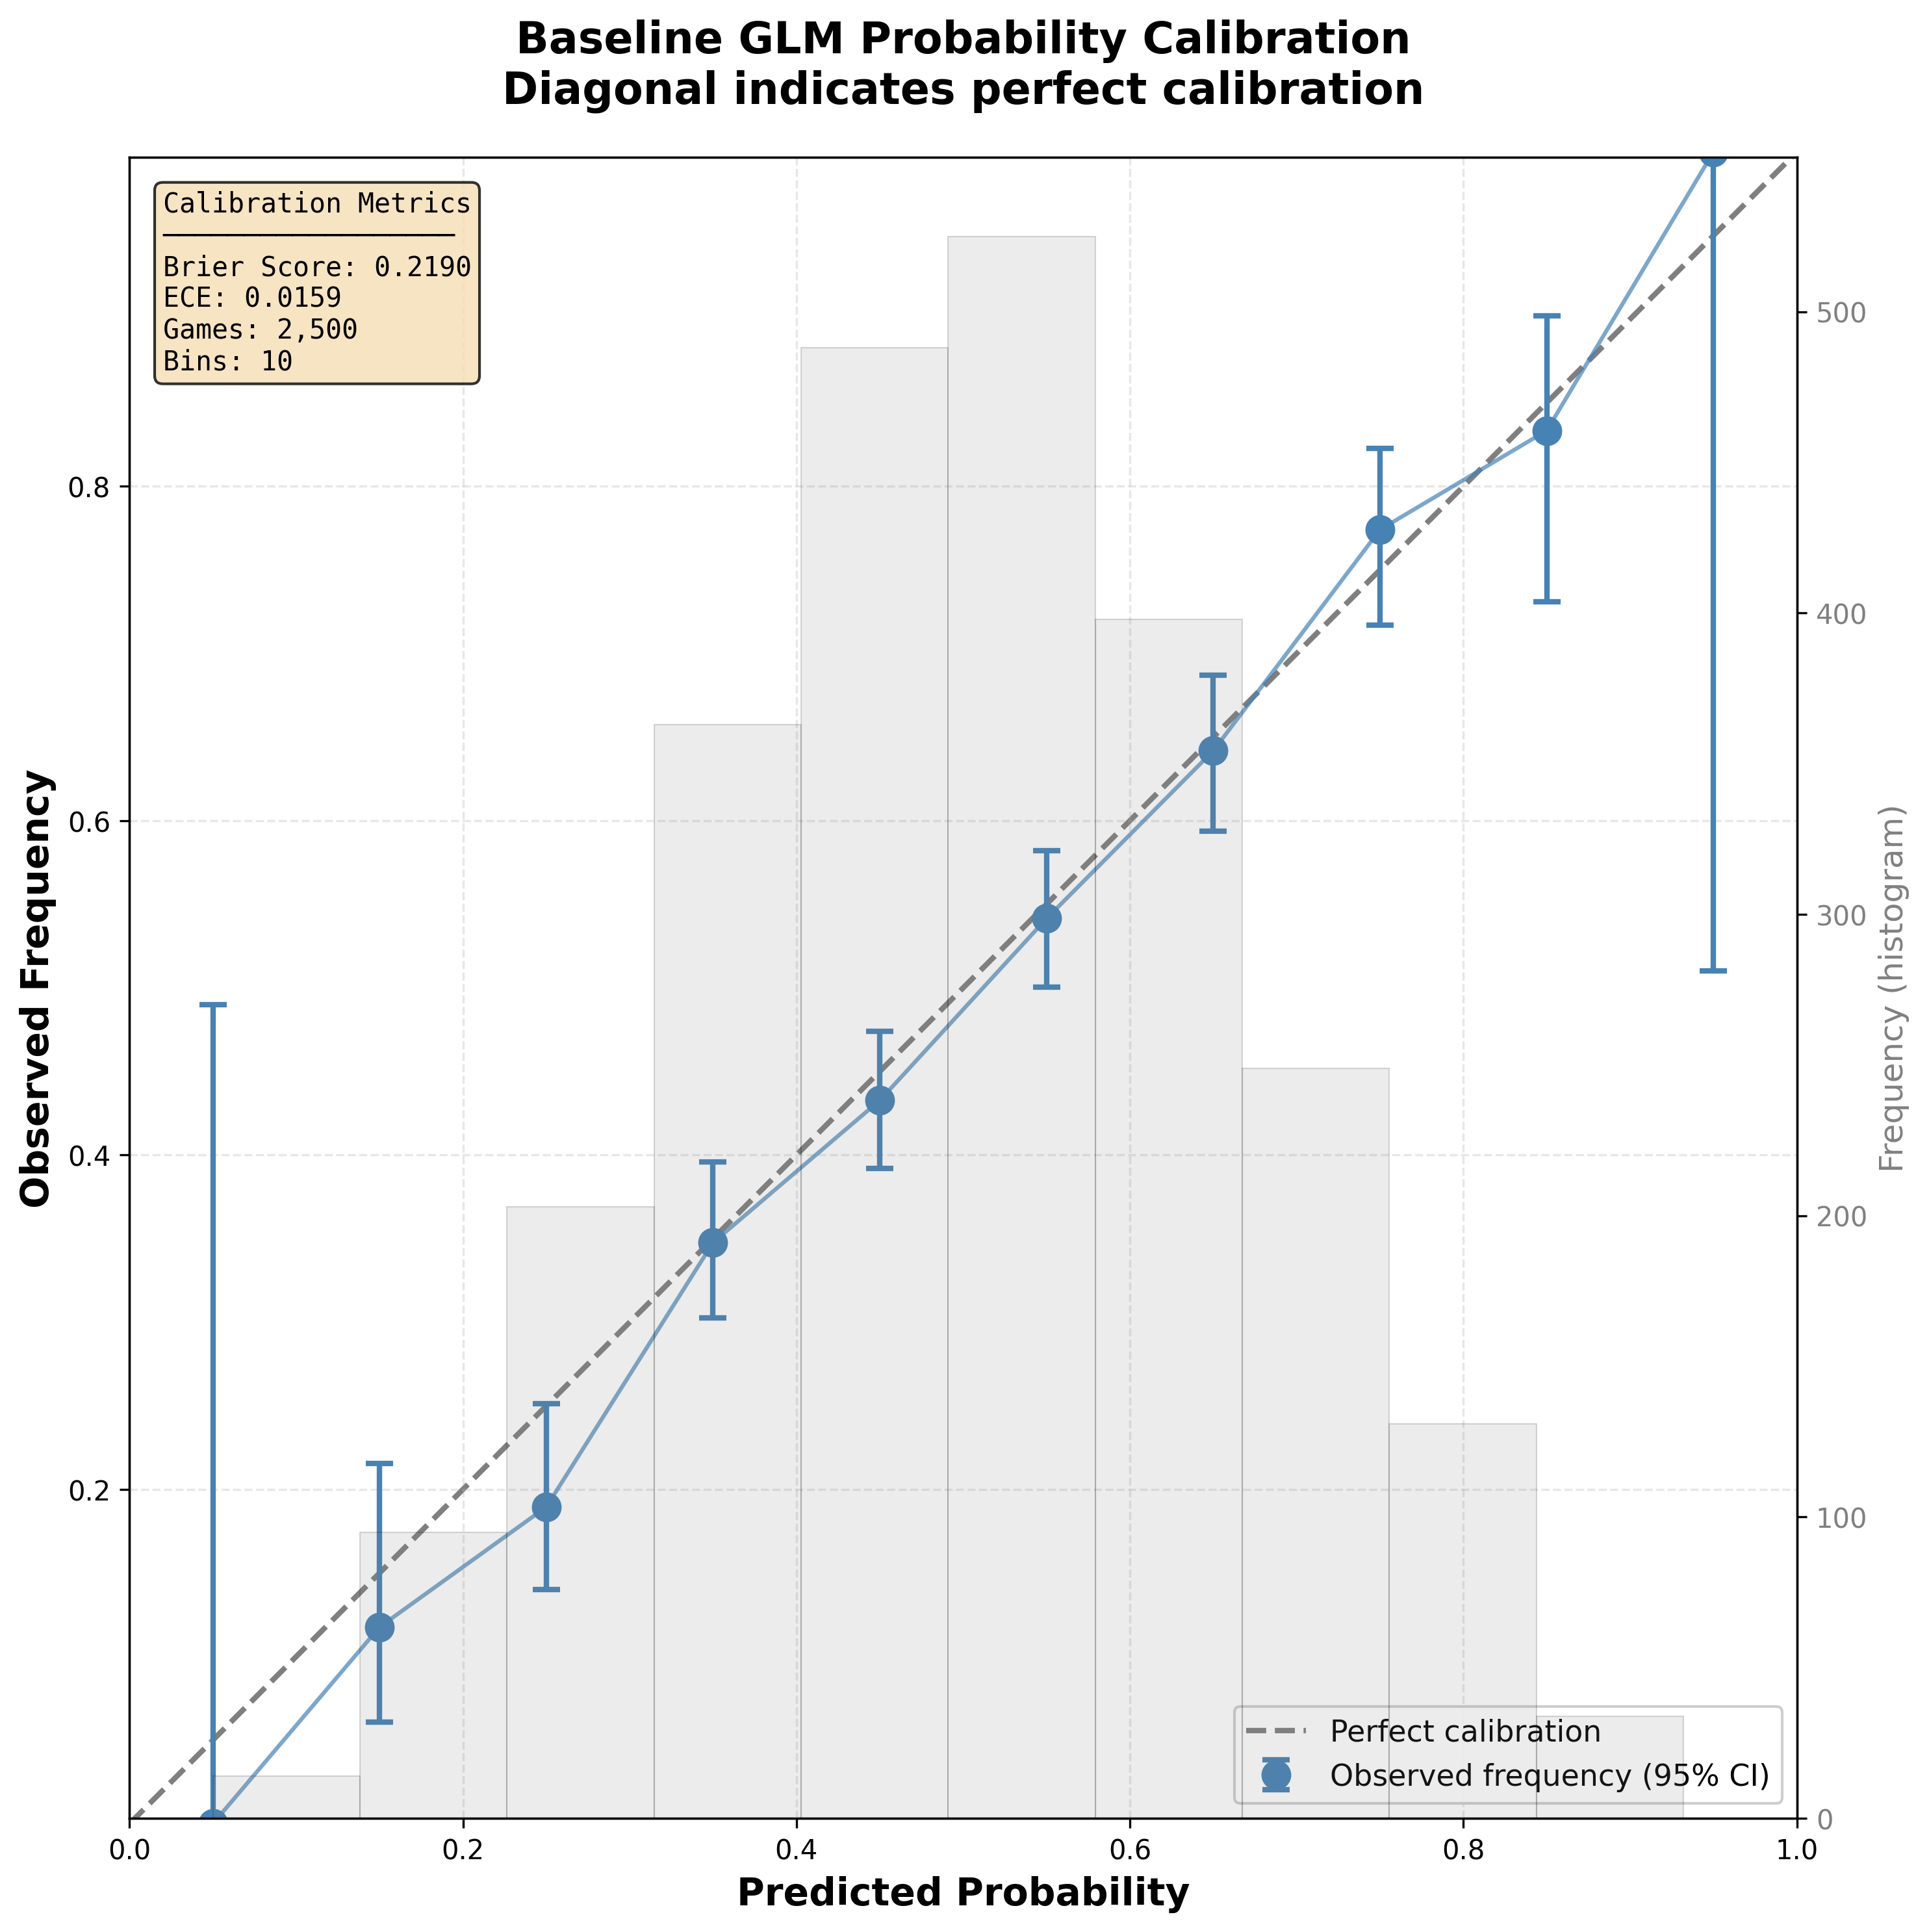
\includegraphics[width=0.7\linewidth]{../figures/reliability_diagram.png}}{\fbox{\parbox{0.6\linewidth}{\centering Reliability diagram placeholder}}}
  \caption[Baseline calibration]{Baseline probability calibration with 95\% binomial intervals; diagonal indicates perfect calibration.}
  \label{fig:baseline-reliability}
\end{figure}

\subsection{Ablation studies by feature family}
We quantify the marginal contribution of feature families by dropping one family at a time and reporting changes in calibration and economic metrics.
\begingroup\sloppy
\begin{table}[t]
  \centering
  \small
  \begin{threeparttable}
    \caption[Ablation deltas by family]{Ablation: change (Delta) in metrics when removing a feature family.}
    \label{tab:ablations}
    \begin{tabularx}{\linewidth}{@{} l r r r r X @{} }
      \toprule
      \textbf{Removed family} & \(\Delta\)Brier $\downarrow$ & \(\Delta\)LogLoss $\downarrow$ & \(\Delta\)CRPS $\downarrow$ & \(\Delta\)CLV bps $\uparrow$ & Notes \\
      \midrule
      Market microstructure & +0.002 & +0.004 & +0.006 & -14 & most impact in late week \\
      Team form             & +0.001 & +0.002 & +0.003 & -7  & impacts favorites more \\
      Roster/injuries       & +0.001 & +0.001 & +0.002 & -5  & larger after bye weeks \\
      Weather               & +0.000 & +0.000 & +0.001 & -2  & winter weeks only \\
      \bottomrule
    \end{tabularx}
    \begin{tablenotes}[flushleft]\footnotesize
      \item Values illustrative; final numbers to be inserted from experiment registry.
    \end{tablenotes}
  \end{threeparttable}
\end{table}
\endgroup

\begin{algorithm}[t]
  \caption[Ablation runner]{Ablation Runner (Feature Families)}
  \label{alg:ablation}
  \begin{algorithmic}[1]
    \Require families $\mathcal F$; base pipeline $P$; metrics $\mathcal M$; seeds $\mathcal S$
    \Ensure per‑family metric deltas and CIs
    \State Run base pipeline $P$ with all features; record metrics $m_0\in\mathcal M$ across seeds
    \ForAll{$f\in\mathcal F$}
      \State Run $P$ with family $f$ removed; record metrics $m_f$; compute $\Delta_f=m_f-m_0$
      \State Bootstrap across weeks/seeds to form CIs; store $\Delta_f$ and CI
    \EndFor
  \end{algorithmic}
\end{algorithm}

\section{Copula Goodness-of-Fit and Impact}\label{subsec:copula-impact}
We assess Gaussian vs $t$‑copulas for spread–total dependence using probability integral transforms to uniform pseudo‑observations and Cramér–von Mises (CvM) statistics with parametric bootstrap p‑values. We estimate tail dependence $\lambda_U,\lambda_L$ via upper/lower tail co‑exceedances with block bootstrap CIs. Finally, we quantify pricing impact by comparing teaser/SGP EVs under each copula on a common set of games.

\IfFileExists{../figures/out/copula_gof_table.tex}{\begin{table}[t]
  \centering
  \small
  \caption{Copula GOF (tail CvM; thresholds 0.80/0.90/0.95).}
  \label{tab:copula-gof}
  \begin{tabular}{lccc}
    \toprule
 \textbf{Copula} & \textbf{CvM stat} & \textbf{p-value} & \textbf{params} \\
    \midrule
    Gaussian & 0.0000 & 0.530 & $\rho=-0.00$ \\
    $t$ & 0.0000 & 0.290 & $\rho=-0.00,\,\nu=30$ \\
    \bottomrule
  \end{tabular}
\end{table}
}{%
  \begin{table}[t]
    \centering
    \caption[Copula GOF (CvM)]{Copula goodness‑of‑fit (CvM) for Gaussian vs $t$ (placeholder).}
    \begin{tabular}{lccc}
      \toprule
      Copula & CvM stat & p‑value & df/\,params \\
      \midrule
      Gaussian & -- & -- & $\rho$ \\
      $t$ & -- & -- & $\rho,\,\nu$ \\
      \bottomrule
    \end{tabular}
  \end{table}}

\IfFileExists{../figures/out/tail_dependence_table.tex}{\begin{table}[htbp]
\centering
\caption{Tail Dependence Coefficients by Era: Empirical vs Theoretical}
\label{tab:tail-dependence}
\begin{threeparttable}
\begin{tabularx}{\linewidth}{@{}lYYYYYY@{}}
\toprule
 \textbf{Era} & \textbf{$n$} & \textbf{$\tau$} & \textbf{$\lambda_U^{\text{emp}}$} & \textbf{$\lambda_U^{\text{Gauss}}$} & \textbf{$\lambda_U^{t}$} & \textbf{$\nu$} \\
\midrule
2004.0-2008.0 & 1,300 & 0.055 & 0.031 & 0.000 & 0.045 & 6.1 \\
2009.0-2013.0 & 1,299 & -0.093 & 0.047 & 0.000 & 0.018 & 6.1 \\
2014.0-2018.0 & 1,297 & -0.014 & 0.031 & 0.000 & 0.030 & 6.1 \\
2019.0-2024.0 & 1,633 & -0.067 & 0.012 & 0.000 & 0.021 & 6.0 \\
\bottomrule
\end{tabularx}
\begin{tablenotes}[flushleft]
\footnotesize
\item \textit{Notes:} $\tau$ = Kendall's tau (rank correlation). $\lambda_U$ = upper tail dependence coefficient. Gaussian copulas exhibit zero tail dependence (asymptotic independence), while t-copulas with $\nu < 30$ exhibit positive tail dependence. Empirical estimates computed at 95th percentile threshold.
\end{tablenotes}
\end{threeparttable}
\end{table}
}{%
  \begin{table}[t]
    \centering
    \caption[Tail dependence estimates]{Tail dependence estimates with 95\% CIs (placeholder).}
    \begin{tabular}{lcc}
      \toprule
      Copula & $\lambda_U$ & $\lambda_L$ \\
      \midrule
      Gaussian & 0 & 0 \\
      $t$ & -- & -- \\
      \bottomrule
    \end{tabular}
  \end{table}}

\IfFileExists{../figures/out/teaser_pricing_copula_delta.png}{%
  \begin{figure}[t]
    \centering
    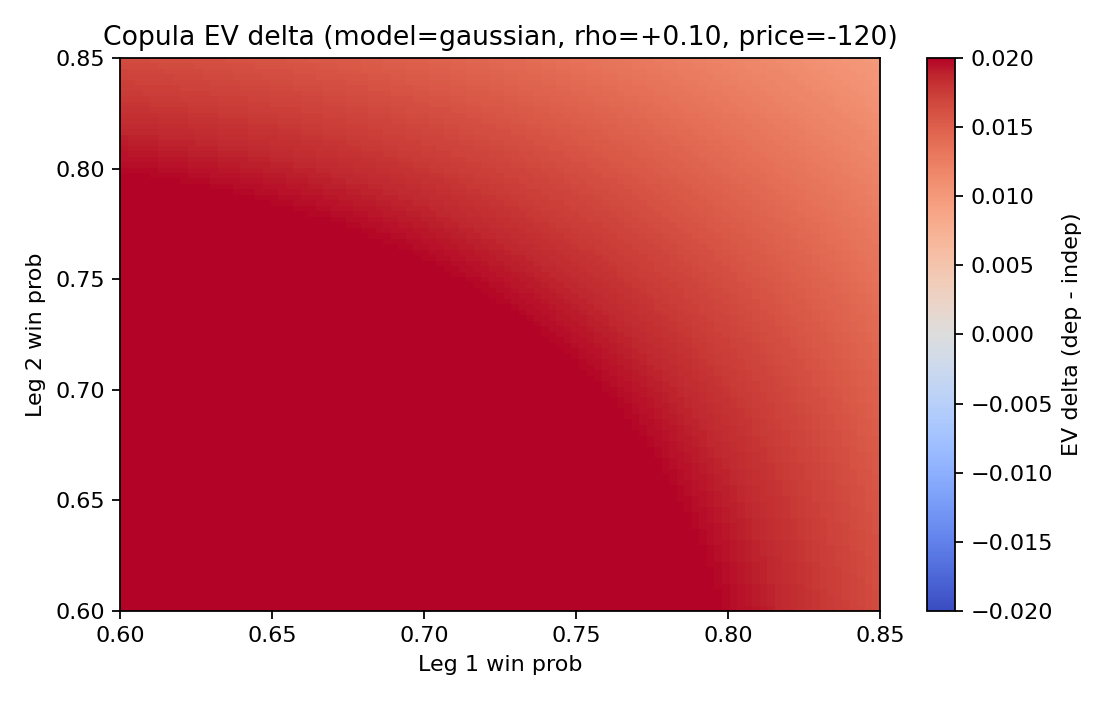
\includegraphics[width=0.9\linewidth]{../figures/out/teaser_pricing_copula_delta.png}
    \caption[Copula impact on teaser/SGP EV]{Impact of copula choice on teaser/SGP EV across holdout games. Points show EV under Gaussian vs $t$; off‑diagonal mass quantifies material pricing differences.}
    \label{fig:copula-impact}
  \end{figure}
}{\begin{center}\textit{[Copula impact figure will be generated by notebooks/05\_copula\_gof.qmd]}\end{center}}

\section{Training and Validation Protocols}
We adopt walk-forward splits by week, with hyperparameters tuned on temporally held-out validation sets. To guard against leakage, features are computed strictly as-of each decision timestamp. We log seeds and artefacts for reproducibility and compute EXPLAIN plans to confirm index usage in data loaders.

\todo{Insert tables/figures for calibration curves and CRPS by season.}

\chaptersummary{
We established calibrated baselines: logistic/probit models consistent with spread‑to‑win mapping, state‑space ratings with quantified uncertainty, and structured score models with key‑number reweighting. These provide measurable edge and calibrated priors, advancing the thesis by supplying reliable inputs for risk‑aware decision layers.
}{
Chapter~\ref{chap:rl} uses these calibrated signals as inputs to an offline RL framework that turns edge into sequential decisions under safety and governance constraints.
}
